\chapter{Конструкторский раздел}

\section{Диаграмма вариантов использования}

На рисунке~\ref{img:use-case} представлена диаграмма вариантов использования.
На основе неё выполним проектировку приложения.

\begin{figure}[H]
	\centering
	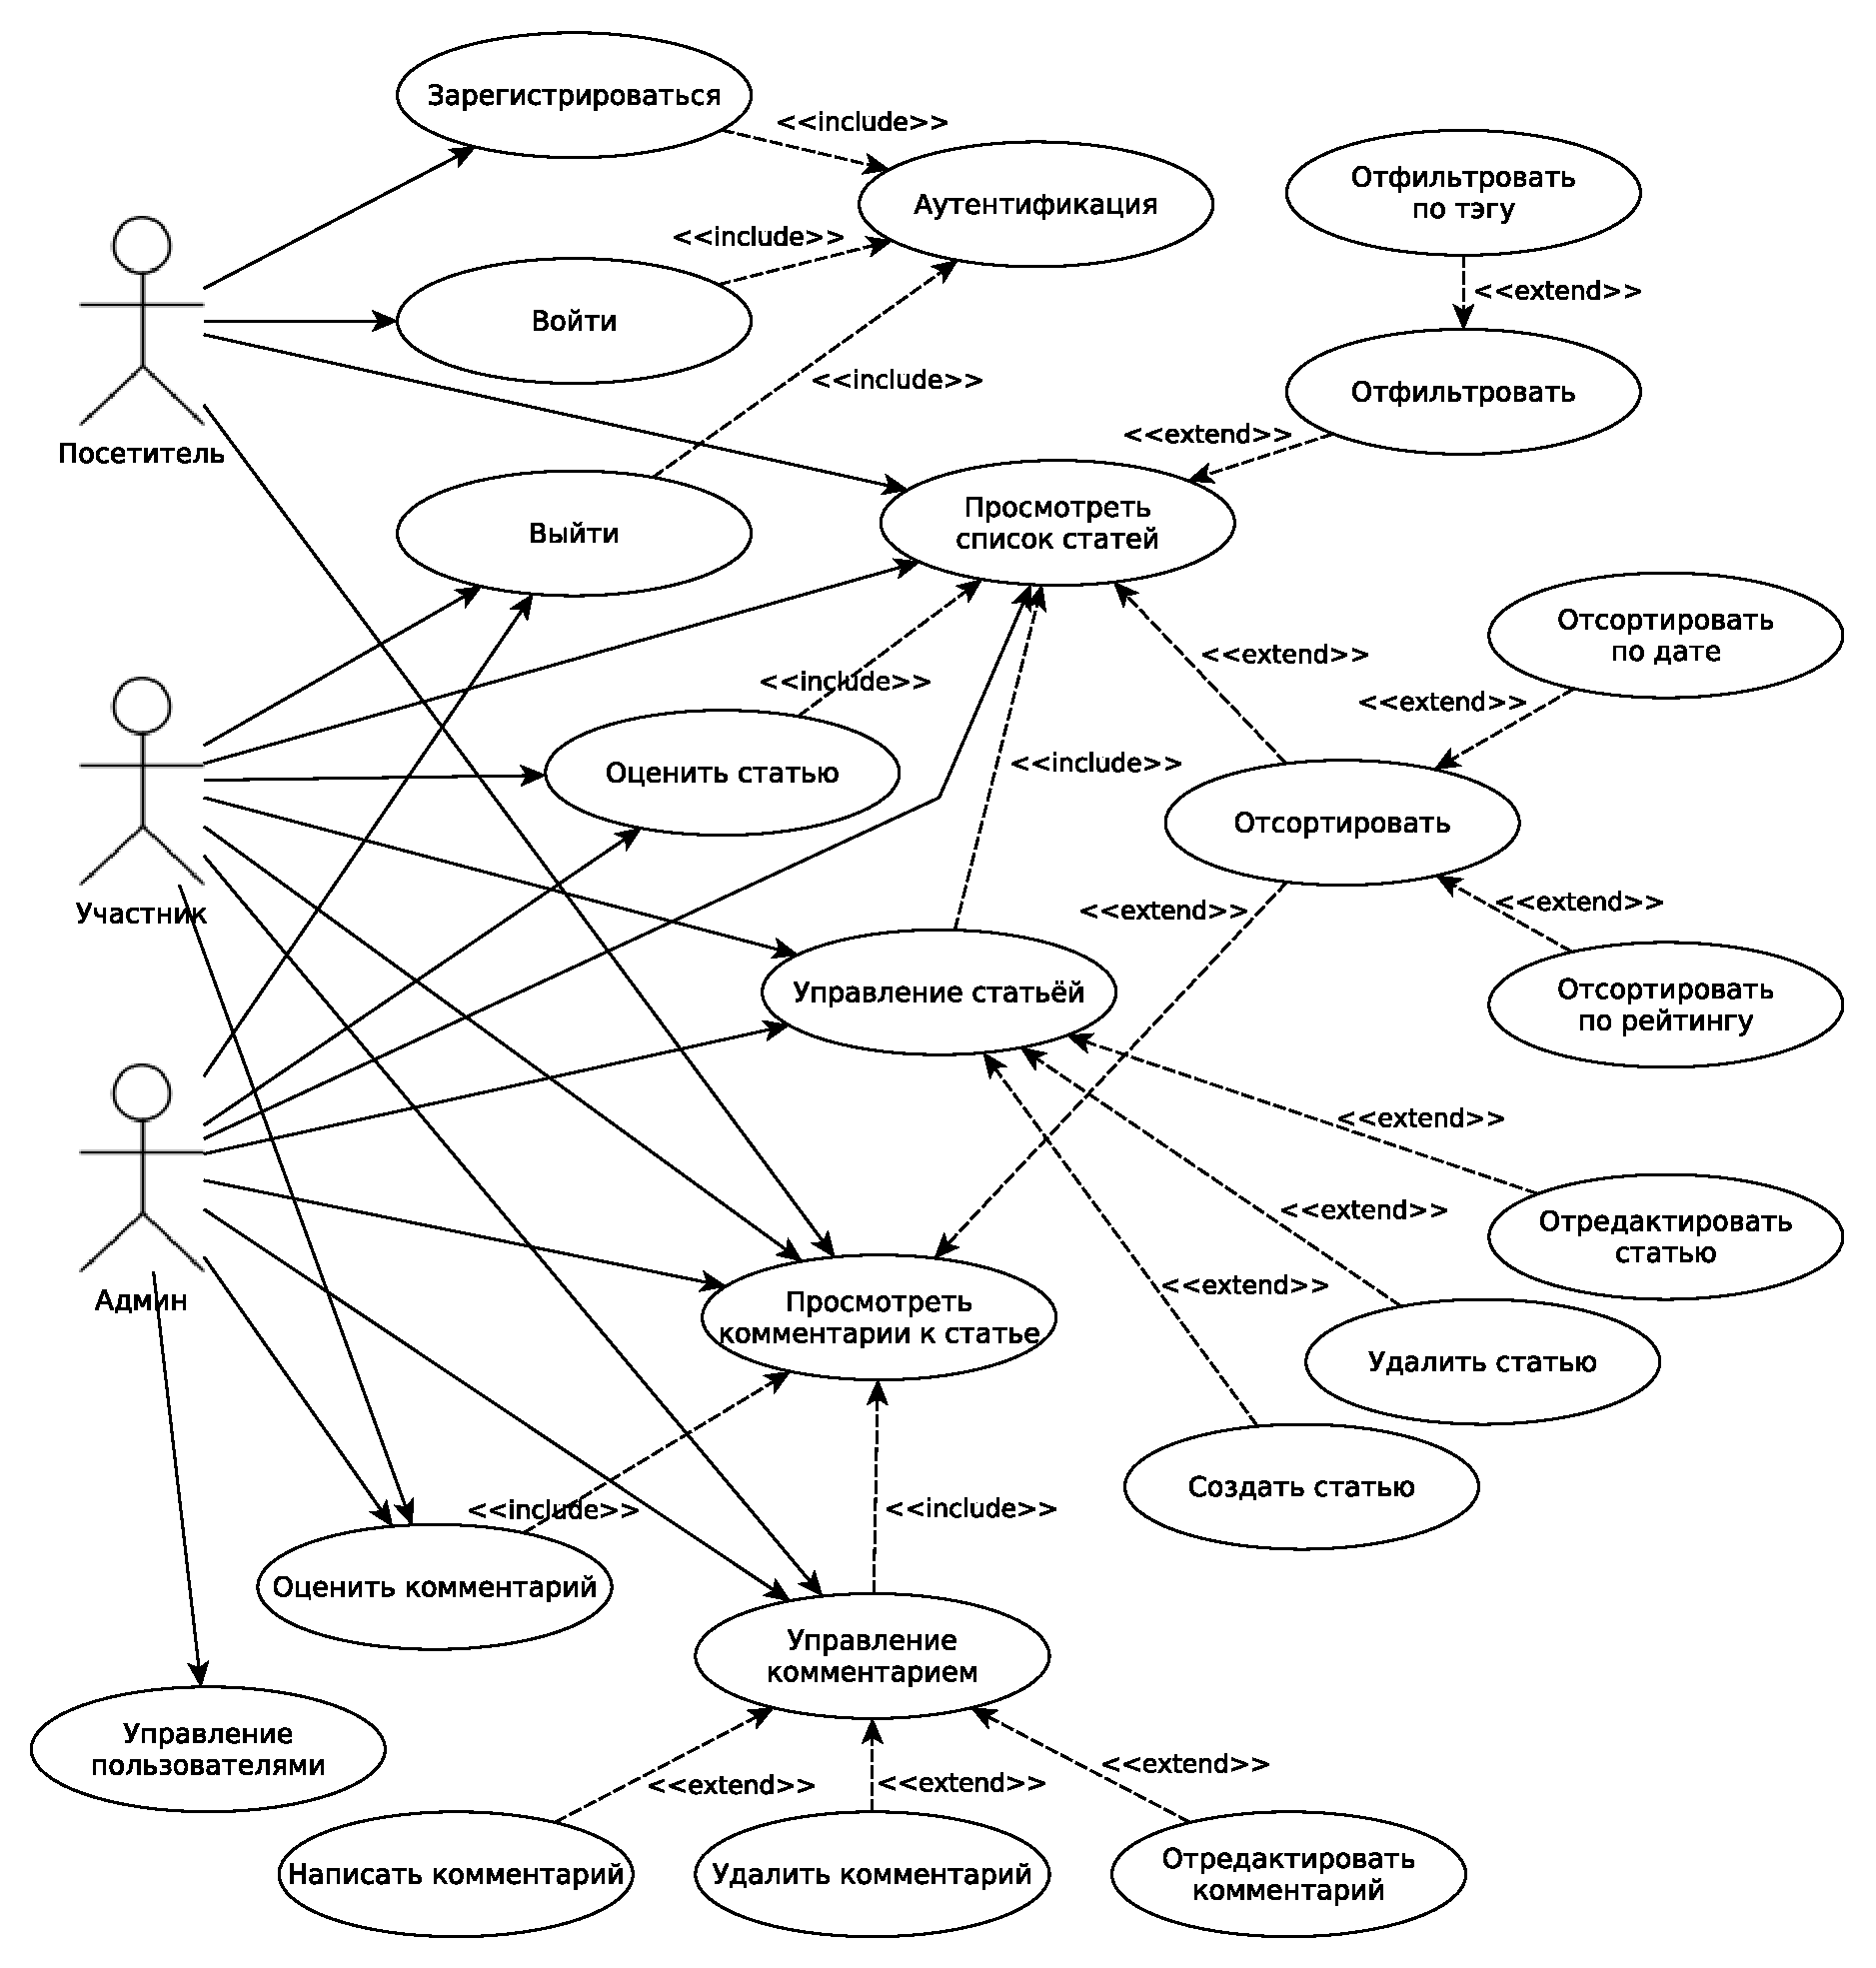
\includegraphics[scale=0.5]{inc/img/use-case}
	\caption{Диаграмма вариантов использования}
	\label{img:use-case}
\end{figure}

\section{Система аутентификации}

Фреймворк Django поставляется с системой аутентификации пользователя.
Она обрабатывает учетные записи пользователей, группы, разрешения и сеансы пользователей на основе файлов cookie.

Система аутентификации Django обрабатывает как аутентификацию, так и авторизацию.
Вкратце, аутентификация подтверждает, что пользователь является тем, кем он себя считает, а авторизация определяет, что разрешено делать аутентифицированному пользователю.
Здесь термин аутентификация используется для обозначения обеих задач.

Наличие встроенной системы аутентификации избавляет от её проектирования.

\section{Структура базы данных}

В данном разделе будут представлены основные таблицы, выделенные в базе данных.

\subsection{Пользователь}

Описание отношения таблицы пользователей User представлено в~таблице~\ref{tbl:auth_user}.
Стоит заметить, что отдельно создавать таблицу, хранящую информацию о пользователях, не придётся: в системе аутентификации фреймворка Django есть стандартная таблица User, отношение которой содержит все нижеперечисленные атрибуты.

\begin{table}[H]
	\centering
	\caption{Отношение таблицы User}
	\label{tbl:auth_user}
	\begin{tabular}{|l|l|l|}
		\hline
		\textbf{Атрибут} & \textbf{Тип} & \textbf{Описание}          \\ \hline
		id               & int          & Идентификатор пользователя \\ \hline
		username         & varchar(150) & Псевдоним пользователя     \\ \hline
		password         & varchar(128) & Пароль                     \\ \hline
		first\_name      & varchar(30)  & Имя                        \\ \hline
		last\_name       & varchar(150) & Фамилия                    \\ \hline
		email            & varchar(254) & Электронная почта          \\ \hline
	\end{tabular}
\end{table}

\subsection{Статья}

Описание отношения таблицы статей Article представлено в~таблице~\ref{tbl:myblog_article}.

\begin{table}[H]
	\centering
	\caption{Отношение таблицы Article}
	\label{tbl:myblog_article}
	\begin{tabular}{|l|l|l|}
		\hline
		\textbf{Атрибут} & \textbf{Тип} & \textbf{Описание}       \\ \hline
		id               & int          & Идентификатор статьи    \\ \hline
		user\_id         & int          & Идентификатор автора    \\ \hline
		title            & varchar(80)  & Заголовок               \\ \hline
		body             & text         & Тело статьи             \\ \hline
		pub\_date        & timestamp    & Дата и время публикации \\ \hline
		rating           & int          & Рейтинг статьи          \\ \hline
	\end{tabular}
\end{table}

\subsection{Комментарий}

Описание отношения таблицы комментариев Comment представлено в~таблице~\ref{tbl:myblog_comment}.

\begin{table}[H]
	\centering
	\caption{Отношение таблицы Comment}
	\label{tbl:myblog_comment}
	\begin{tabular}{|l|l|l|}
		\hline
		\textbf{Атрибут} & \textbf{Тип} & \textbf{Описание}                   \\ \hline
		id               & int          & Идентификатор комментария           \\ \hline
		user\_id         & int          & Идентификатор автора комментария    \\ \hline
		article\_id      & int          & Идентификатор комментируемой статьи \\ \hline
		body             & text         & Текст комментария                   \\ \hline
		pub\_date        & timestamp    & Дата и время публикации комментария \\ \hline
		rating           & int          & Рейтинг комментария                 \\ \hline
	\end{tabular}
\end{table}

\subsection{Тэг}

Описание отношения таблицы тэгов Tag представлено в~таблице~\ref{tbl:myblog_tag}.

\begin{table}[H]
	\centering
	\caption{Отношение таблицы Tag}
	\label{tbl:myblog_tag}
	\begin{tabular}{|l|l|l|}
		\hline
		\textbf{Атрибут} & \textbf{Тип} & \textbf{Описание}  \\ \hline
		id               & int          & Идентификатор тэга \\ \hline
		tag              & varchar(50)  & Тэг                \\ \hline
	\end{tabular}
\end{table}

\subsection{Голоса}

Описание отношения таблицы голосов Vote представлено в~таблице~\ref{tbl:myblog_vote}.
Подразумевается, что проголосовать пользователи могут как за статью, так и за комментарий.
Поэтому, чтобы не создавать две отдельные таблицы голосов, введём атрибут content\_type\_id, меняя значение которого можно голосовать за разный тип контента (статьи, голоса).
Идентификатор object\_id будет ссылаться на запись в таблице с идентификатором типа контента content\_type\_id.
Фреймворк Django по умолчанию индексирует каждую созданную таблицу и добавляет новую запись в таблицу типов контентов, описание отношения которой представлено в таблице \ref{tbl:django_content_type}.

\begin{table}[H]
	\centering
	\caption{Отношение таблицы Vote}
	\label{tbl:myblog_vote}
	\begin{tabular}{|l|l|l|}
		\hline
		\textbf{Атрибут}  & \textbf{Тип} & \textbf{Описание}                           \\ \hline
		id                & int          & Идентификатор голоса                        \\ \hline
		user\_id          & int          & Идентификатор проголосовавшего пользователя \\ \hline
		value             & smallint     & Значение ($+1$ или $-1$)                    \\ \hline
		object\_id        & int          & Идентификатор объекта                       \\ \hline
		content\_type\_id & int          & Идентификатор типа контента                 \\ \hline
	\end{tabular}
\end{table}

\begin{table}[H]
	\centering
	\caption{Отношение таблицы content\_type}
	\label{tbl:django_content_type}
	\begin{tabular}{|l|l|l|}
		\hline
		\textbf{Атрибут} & \textbf{Тип} & \textbf{Описание}           \\ \hline
		id               & int          & Идентификатор типа контента \\ \hline
		app\_label       & verchar(100) & Название приложения         \\ \hline
		model            & verchar(100) & Название модели             \\ \hline
	\end{tabular}
\end{table}

\section*{Вывод}

Была представлена диаграмма вариантов использования, с помощью которой была спроектирована база данных, обеспечивающая возможность пользователей аутентифицироваться, создавать, редактировать и оценивать статьи и комментарии к ним.
